%% You can use this file to create your answer for Exercise 1.  
%% Fill in the places labeled by comments.
%% Generate a PDF document by with the command `pdflatex ex1'.

\documentclass[11pt]{article}

\usepackage{fullpage}
\usepackage{amsmath,amsopn}
\usepackage{graphicx}
\usepackage{color}
\usepackage{verbatim}
\usepackage{setspace}
\usepackage{gensymb}
\usepackage{float}
\usepackage{pgfplots}
\pgfplotsset{compat=1.16}
\usepackage[normalem]{ulem}
%\usepackage[dvips,bookmarks=false,colorlinks,urlcolor=blue,pdftitle={
\usepackage{caption}
\usepackage{subcaption}
\usepackage{amssymb}
\usepackage{amsfonts}
\usepackage{amsthm}
\usepackage{comment}
\usepackage{times}
\usepackage{listings}
\usepackage{enumerate}
\usepackage{courier}
\usepackage{hyperref}
\usepackage{xcolor}
\usepackage{verbatimbox}
\usepackage{tikz}
\usepackage{tikzscale}
\usepgfplotslibrary{groupplots}
\usepackage{float}
\usepackage{natbib}

\def\vO{{\bf O}}
\def\vP{{\bf P}}
\def\vp{{\bf p}}
\def\vx{{\bf x}}
\def\vl{{\bf l}}
\def\mS{{\bf S}}
\def\mT{{\bf T}}
\def\mH{{\bf H}}
\def\mA{{\bf A}}
\def\tx{{\tilde{\bf x}}}
\def\ta{{\tilde{\bf a}}}
\def\tb{{\tilde{\bf b}}}
\def\tc{{\tilde{\bf c}}}
\def\hn{{\bf \hat{n}}}
\def\hv{{\bf \hat{v}}}
\def\hh{{\bf \hat{h}}}
\def\vh{{\bf h}}
\def\vs{{\bf s}}
\def\hs{{\bf \hat{s}}}
\newcommand{\R}{\mathbb{R}}
\newcommand{\ud}{\,\mathrm{d}}

%% Values that are specific to a particular term
\newcommand{\thisterm}{Fall 2023}

\newcommand{\dateassigned}{Wed., Sep. 13}

%% Printed form of home page that students should use
\newcommand{\visiblecoursehome}{http://www.cs.cmu.edu/\textasciitilde{}418}

%% Link to home page that will stay valid
\newcommand{\actualcoursehome}{http://www.cs.cmu.edu/afs/cs.cmu.edu/academic/class/15418-s23/www}

\newcommand{\datedueregistered}{Wed.,~Sep.~27}

%% Page layout
\oddsidemargin 0pt
\evensidemargin 0pt
\textheight 600pt
\textwidth 469pt
\setlength{\parindent}{0em}
\setlength{\parskip}{1ex}

%% Colored hyperlink 
\newcommand{\cref}[2]{\href{#1}{\color{blue}#2}}
\newcommand{\todo}[1]{[\textcolor{red}{\textit{TODO: }{#1}}]}

%% Customization to listing
\lstset{basicstyle=\ttfamily,language=C++,morekeywords={uniform,foreach}}

%% Enumerate environment with alphabetic labels
\newenvironment{choice}{\begin{enumerate}[A.]}{\end{enumerate}}
%% Environment for supplying answers to problem
\newenvironment{answer}{\begin{minipage}[c][1.0in]{\textwidth}}{\end{minipage}}
\newenvironment{answer2}{\begin{minipage}[c][1.0in]{\textwidth}}{\end{minipage}}

\begin{document}
\begin{center}
\LARGE
15-418/618 \thisterm{} Final Project Proposal
\\ 
Sparse Attention in CUDA
\end{center}
\begin{flushright}
{\large\bf Full Names: Sarah Di, Jinsol Park\makebox[2in][l]{
%% Put your name on the next line

}}

{\large\bf Andrew IDs: sarahdi, jinsolp\makebox[2in][l]{\tt
%% Put your Andrew ID on the next line

}}
\end{flushright}

{\large\bf Project Page URL: \url{https://github.com/disarah/15618\_Project}\makebox[2in][l]{
%% Put your name on the next line

}}

% Highlight attention matters in performance
% execution time of attention vs execution of other layers
% attention dominates computation
% optimizing important components

% bottleneck of performance

\section{Summary}
We are going to implement sparse attention on CPU and GPU platforms using python and CUDA respectively, and perform analysis on both system's performance characteristics.

% (2-3 sentences) Describe what you plan to do and what parallel systems you will be working with. Example one-liners include (you should add a bit more detail):

% • We are going to implement an optimized Smoothed Particle Hydrodynamics fluid solver on the NVIDIA GPUs in the lab.
% • We are going port the Go runtime to Blacklight.

% • We are going to create optimized implementations of sparse-matrix multiplication on both GPU and multi-core CPU platforms, and perform a detailed analysis of both systems’ performance characteristics.

% • We are going to back-engineer the unpublished machine specifications of the GPU in the tablet my partner just purchased.

% • We are going to implement two possible algorithms for a real-time computer vision application on a mobile device and measure their energy consumption in the lab.

\section{Background}
% \subsection{Attention being a bottleneck of Transformers}
Attention requires time and memory that that scales quadratically with sequence length \cite{child2019generating}.

% \subsection{Sparse Attention}
Sparse attention is similar to the original attention, but it factorizes the attention matrix to compute certain parts of the matrix instead of computing the entire $n \times n$ matrix. Different factorization methods lead to different sparse attention modes.

\begin{figure}[h]
  \centering
  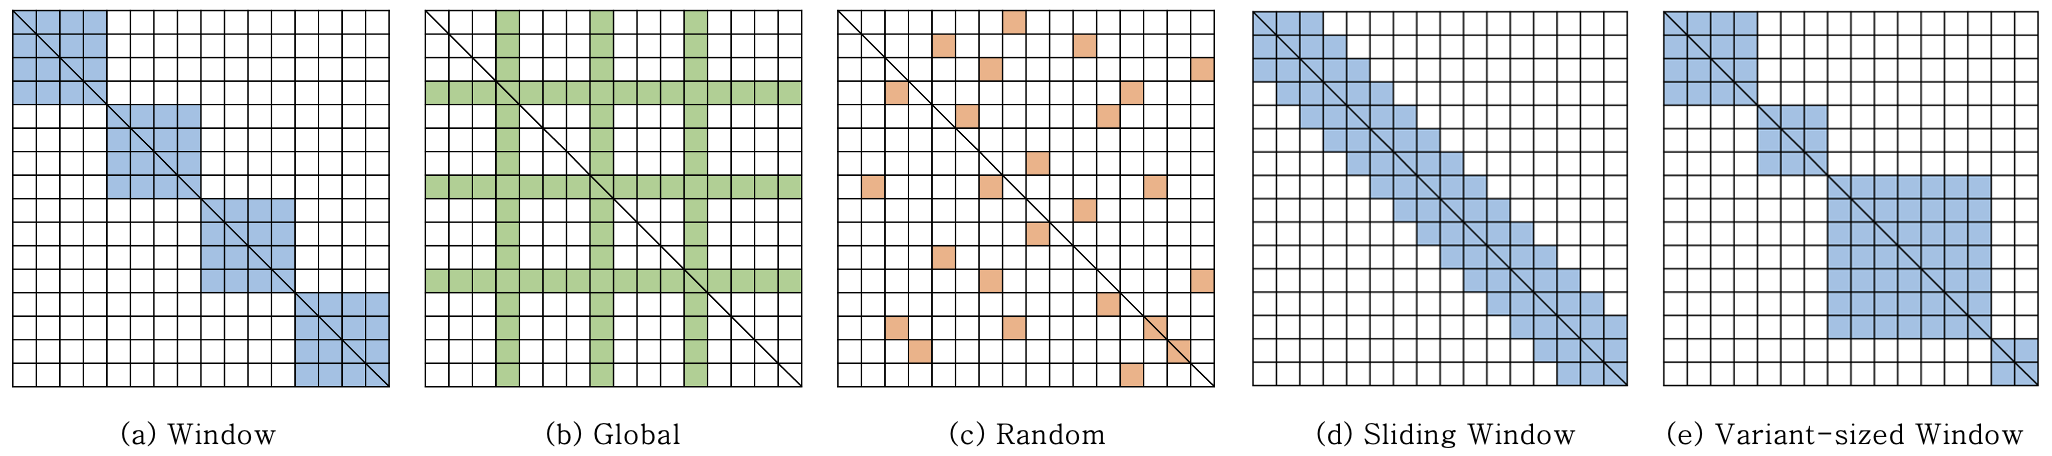
\includegraphics[width=170mm]{figures/building_block.png}
  \caption{Different factorization methods of sparse attention.  Each connectivity matrix shows whether an $i^{th}$ token (row) of a sequence refers to a $j^{th}$ token (column) to compute an attention score. These can be combined to be a single sparse attention method.}
 \label{fig:bulding_block}
\end{figure}

\autoref{fig:bulding_block} illustrates different sparse attention factorization methods. 
We think that instead of naively implementing this by checking every element, parallelizing matrix multiplication by taking sparsity into account will be important for gaining high speedup. Thus, we are planning to implement CPU and GPU versions of sparse attention by actually checking only the elements that matter, which are decided in advance by user configurations.
Based on this implementation, we are planning to analyze how much speedup sparse attention brings compared to naive matrix multiplication.

% If your project involves accelerating a compute-intensive application, describe the application or piece of the application you are going to implement in more detail. It might be helpful to include a block diagram or pseudocode of the basic idea. An important detail is what aspects of the problem might benefit from parallelism and why?

% Describe Sparse Attention (a few paragraphs)
% Include Sparse Attention graph thing

% - Attention takes up a large portion of Transformers (in terms of computation time)
% Using CUDA - parallelize matrix multiplication aspect of sparse attention + analyze how much speedup (?) using sparse attention brings compared to naive matmul.

\section{The Challenge}
First, implementing sparse attention in CUDA itself is challenging. As aforementioned, we are planning to consider sparsity itself when doing matrix multiplication. This means that we will be looking at elements in certain strides under different configurations. The main aspect that needs to be considered when implementing sparse attention will be locality. Since we will essentially be performing sparse matrix multiplication under a certain rule, exploiting shared memory will become much more complex compared to naive matrix multiplication.

Also, we plan to implement different sparse attention methods and analyze them against the CPU version. We believe that profiling the execution time and the kernel in detail will also be challenging.

Overall, we wish to deepen our understanding of attention and how matrix multiplication can be parallelized, while also learning how to exploit shared memory on CUDA.

% Describe why the problem is challenging. What aspects of the problem might make it difficult to parallelize? In other words, what to you hope to learn by doing the project?

% • Describe the workload: what are the dependencies, what are its memory access characteristics? (is there locality? is there a high communication to computation ratio?), is there divergent execution?

% • Describe constraints: What are the properties of the system that make mapping the workload to it challenging?

% - implementing sparse attention itself is challenging (different configurations, strides, ....)
% - optimizing sparse matrix multiplication using shared memory exploiting the characteristics (?) GPU - considering warps?? adjust block size or something...
% We hope to learn even more about CUDA

\section{Resources}
\subsection{Tutorials}
We plan to start by looking into the following sparse attention tutorials in DeepSpeed.
\begin{itemize}
    \item \url{https://www.deepspeed.ai/tutorials/sparse-attention/}
    \item \url{https://github.com/microsoft/DeepSpeed/tree/master/deepspeed/ops/sparse\_attention}
\end{itemize}

Also, since we are planing to use the C++ front-end of PyTorch to make it compatible with our custom CUDA kernels, we plan to look into the following C++ PyTorch tutorial.
\begin{itemize}
    \item \url{https://pytorch.org/tutorials/advanced/cpp_frontend.html}
\end{itemize}

% Also, since we are planning to use PyTorch as the main framework, and use our own CUDA kernels for the attention part, we also plan to look into the following tutorial to make customized CUDA kernels as PyTorch Ops.
% \begin{itemize}
%     \item \url{https://pytorch.org/tutorials/advanced/cpp_extension.html}
% \end{itemize}

\subsection{Code Base}
We plan to implement our own Attention module in C++ using PyTorch C++ front-end APIs.
To analyze the bottleneck of attention within the entire transformers layer, we plan to use the Huggingface Transformers library, and run a simple model.


% We plan to implement our own code in PyTorch by referencing the original PyTorch Attention module.

\subsection{Papers}
We plan to read and refer to the following papers; \citet{vaswani2017attention, child2019generating, beltagy2020longformer, zaheer2020big}

% \begin{itemize}
% \itemsep 0em
%     \item Vaswani, Ashish, et al. "Attention is all you need." Advances in neural information processing systems 30 (2017).
%     \item Child, Rewon, et al. "Generating long sequences with sparse transformers." arXiv preprint arXiv:1904.10509 (2019).
%     \item Beltagy, Iz, Matthew E. Peters, and Arman Cohan. "Longformer: The long-document transformer." arXiv preprint arXiv:2004.05150 (2020).
%     \item Zaheer, Manzil, et al. "Big bird: Transformers for longer sequences." Advances in neural information processing systems 33 (2020): 17283-17297.
% \end{itemize}


% Describe the resources (type of computers, starter code, etc.) you will use. What code base will you start from? Are you starting from scratch or using an existing piece of code? Is there a book or paper that you are using as a reference (if so, provide a citation)? Are there any other resources you need, but haven’t figured out how to obtain yet? Could you benefit from access to any special machines?

% Mention starting with the DeepSpeed tutorials/implementation of sparse attention
% https://www.deepspeed.ai/tutorials/sparse-attention/
% https://github.com/microsoft/DeepSpeed/tree/master/deepspeed/ops/sparse\_attention 

% + cite a few sparse attention papers 

\section{Goals and Deliverables}
\subsection{Goals}

\textbf{Plan to Achieve}
\begin{itemize}
\itemsep 0em
    \item Read related papers and work on tutorials to deepen our understanding
    \item Implement sparse attention on CPU
    \item Implement sparse attention on GPU using CUDA
    \item Optimize GPU version of sparse attention by exploiting shared memory
    \item Analyze the speedup gains of sparse attention against naive attention, and also observe different gains on CPU vs GPU.
    \item Analyze different input sequence lengths to observe larger gains with longer sequence lengths.
\end{itemize}


\textbf{Hope to Achieve}
\begin{itemize}
\itemsep 0em
    \item Implement multiple versions of sparse attention, and compare their performance gains.
    \item Profile our sparse attention CUDA kernel with Nsight Compute to find room for further optimization.
\end{itemize}

% • Separate your goals into what you PLAN TO ACHIEVE (what you believe you must get done to have a successful project and get the grade you expect) and an extra goal or two that you HOPE TO ACHIEVE if the project goes really well and you get ahead of schedule, as well as goals in case the work goes more slowly. It may not be possible to state precise performance goals at this time, but we encourage you be as precise as possible. If you do state a goal, give some justification of why you think you can achieve it. (e.g., I hope to speed up my starter code 10x, because if I did it would run in real-time.)

% \textbf{Goals}
% \begin{enumerate}
%     \item Plan to achieve
%     \item Hope to achieve
% \end{enumerate}
% Plan to achieve
% - read papers + do tutorials
% - working sparse attention implmentation (cpu)
% - working sparse attention implmentation (CUDA)
% ===================================
% <- different ver of sparse attention
% - optimize using shared memory

% Hope to achieve
% ====================================
% - profile the kernels in detail using nsight compute
% - compare multiple sparse attention modes 

\subsection{Deliverables}
At the poster session we will be showing speedup graphs. 
We plan to plot these graphs to show speedup against the naive matrix multiplication, and also to show different gains between CPU and GPU.
We also plan to show different speedup gains depending on different sequence lengths. We hope to verify that sparse attention brings significant speedup compared to the original matrix multiplication.

% Mention something about analyzing sparse attention + ways we can bring speedup

% • If your project is an analysis project, what are you hoping to learn about the workload or system being studied? What question(s) do you plan to answer in your analysis?


\section{Platform Choice}
% Describe why the platform (computer and/or language) you have chosen is a good one for your needs. Why does it make sense to use this parallel system for the workload you have chosen?


We plan to implement our own CUDA kernels for sparse attention.
Also, we plan to use the C++ front-end of PyTorch to build our deep learning models since it is easy to use and directly compatible with CUDA kernels (so we also do not have to make python - C++ bindings).
% Thus, we are going to use python-C++ bindings provided by Torch so that we can call our CUDA kernels in the Python environment.

% We plan to used PyTorch since it is easy to use when building deep learning models.
% However, we also plan to implement our own CUDA kernels for sparse attention.
% Thus, we are going to use python-C++ bindings provided by Torch so that we can call our CUDA kernels in the Python environment.

% - CUDA (C++/C)
% - PyTorch/T + CUDA kernels -> python-C binding so that we can call the CUDA kernels

% https://pytorch.org/cppdocs/

\section{Schedule}
Our planned schedule is as follows:
\begin{center}
\begin{tabular}{ |c|c| } 
 \hline
 Time & Plan \\ 
 \hline
 11/15 & Project Proposal Due \\
 11/19 & Work on tutorials, understanding sparse attention\\
 - & Get used to C++ frontend for PyTorch \\
 11/26 & Create CPU implementation\\
 12/03 & Milestone Report Due \\ 
 - & Have 1 CUDA implementation \& benchmark\\
 12/10 & Additional CUDA implementations \& optimizations\\
 12/14 & Final Report Due \\ 
 12/15 & Poster Session \\
 \hline
\end{tabular}
\end{center}
\bibliographystyle{unsrtnat}
\bibliography{ProposalReport/proposal}
\end{document}